\documentclass{beamer}
\usepackage[utf8]{inputenc}
\usepackage{amsmath}
\usepackage{amsthm}
\usepackage{amsfonts}
\usepackage{hyperref}
\usepackage{subcaption}
\usepackage{graphicx}

\DeclareMathOperator{\Tr}{Tr}
\DeclareMathOperator{\dom}{dom}
\DeclareMathOperator{\diag}{diag}
\DeclareMathOperator{\dist}{dist}
\DeclareMathOperator{\spn}{span}
\DeclareMathOperator{\prob}{P}
\DeclareMathOperator{\E}{E}
\DeclareMathOperator{\conv}{conv}
\DeclareMathOperator*{\argmax}{arg\,max}
\DeclareMathOperator*{\argmin}{arg\,min}

\newcommand{\norm}[1]{\lVert#1\rVert}
\newcommand{\ceil}[1]{\left\lceil#1\right\rceil}
\newcommand{\floor}[1]{\left\lfloor#1\right\rfloor}

\title{Signed Support Recovery with the LASSO}
\author{Benjamin Noland}
\date{}

%\usetheme{Madrid}

\begin{document}

\frame{\titlepage}

\begin{frame}
\frametitle{Background}

Common problem: Want to estimate parameter vector
$\beta^\ast \in \mathbb{R}^p$ in the linear model
\begin{equation*}
  y = X\beta^\ast + \epsilon,
\end{equation*}
where
\begin{itemize}
\item $y \in \mathbb{R}^n$ is a vector of observed responses,
\item $X \in \mathbb{R}^{n \times p}$ is the design matrix, and
\item $\epsilon \in \mathbb{R}^n$ is a zero-mean random vector
  representing the uncertainty in the model.
\end{itemize}

\end{frame}

\begin{frame}
\frametitle{Background}

\begin{itemize}
\item Problem is easy to solve in the \textit{classical setting}:
  $p \leq n$. Simple linear algebra.
\item Not so well understood when $p > n$. Case belongs to the active
  area of research known as \textit{high-dimensional statistics}.
\end{itemize}

\end{frame}

\begin{frame}
\frametitle{What to do when $p > n$?}

\begin{itemize}
\item Assume the data is \textit{truly low-dimensional}, i.e, that lot
  of the entries in $\beta^\ast$ are actually zero.
\item Define the \textit{support} of $\beta^\ast$ by
\begin{equation*}
  S(\beta^\ast) = \{i \in \{1, \ldots, p\} : \beta^\ast_i \neq 0\},
\end{equation*}
and let $k = |S(\beta^\ast)|$.
\item Assume that $k \ll p$ (a \textit{sparsity assumption} on
  $\beta^\ast$).
\item Want to compute $S(\beta^\ast)$ to identify which variables are
  truly important.
\end{itemize}

\end{frame}

\begin{frame}
\frametitle{The LASSO}

A computationally tractible method for computing $\beta^\ast$ in the
high-dimensional setting is the \textit{LASSO} (Least Absolute
Shrinkage And Selection Operator):
\begin{equation*}
  \begin{array}{ll}
    \text{minimize} & \norm{y - X\beta}_2^2 \\
    \text{subject to}
      & \norm{\beta}_1 \leq C_n
  \end{array},
\end{equation*}
where $C_n > 0$, or equivalently, as the solution to the unconstrained
problem
\begin{equation*}
  \text{minimize} \
    \frac{1}{2n} \norm{y - X\beta}_2^2 + \lambda_n \norm{\beta}_1,
\end{equation*}
where $\lambda_n \geq 0$ is a \textit{regularization parameter} that
is in one-to-one correspondence with $C_n$ via Lagrangian duality.

\end{frame}

\begin{frame}
\frametitle{Project overview}

\begin{itemize}
\item Restrict attention to random designs $X$.
\item Explore the contributions of the following paper to support
  recovery using the LASSO:
  \begin{flushleft}
    Wainwright, M. (2006).
    \textit{Sharp thresholds for high-dimensional and noisy sparsity
      recovery using $l_1$-constrained quadratic programming (Lasso)}.
    Technical Report 709, Dept. Statistics, Univ. California, Berkeley
  \end{flushleft}
\item See what happens when we replace the LASSO $l_1$-penalty term
  with a more general \textit{elastic net} penalty
  \begin{equation*}
    \lambda_n \left( \frac{1}{2} (1 - \alpha) \norm{\beta}_2^2
      + \alpha \norm{\beta}_1 \right ),
  \end{equation*}
  where $\alpha \in [0, 1]$.
\item Conduct simulations and look at the results.
\end{itemize}

\end{frame}

\begin{frame}
\frametitle{Signed support recovery}

\begin{itemize}
\item Results from Wainwright paper provide necessary and sufficient
  conditions for the LASSO to recover the \textit{signed support} of
  $\beta^\ast$ with high probability.
\item \textit{Signed support} $\mathbb{S}_\pm(\beta)$ of
  $\beta \in \mathbb{R}^p$:
\begin{equation*}
  \mathbb{S}_\pm(\beta)_i =
  \begin{cases}
    +1 & \quad \text{if $\beta_i > 0$} \\
    -1 & \quad \text{if $\beta_i < 0$} \\
    0 & \quad \text{if $\beta_i = 0$}
  \end{cases}
  \quad (i = 1, \ldots, p).
\end{equation*}
\item Questions:
  \begin{itemize}
  \item What relationships between $n$, $p$, and $k$ yield a
    \emph{unique} LASSO solution $\hat{\beta}$ satisfying
    $\mathbb{S}_\pm(\hat{\beta}) = \mathbb{S}_\pm(\beta^\ast)$?
  \item For what relationships between $n$, $p$, and $k$ does \emph{no
      solution} of the LASSO yield the correct signed support?
  \end{itemize}
Considered for both deterministic and random designs $X$.

\end{itemize}

\end{frame}

\begin{frame}
\frametitle{Results from Wainwright paper}

\begin{itemize}
\item Will quickly sketch out results from Wainwright paper for case
  of random design.
\item Too much notation to define everything here. \textbf{See the
    paper!}
\end{itemize}

\end{frame}

\begin{frame}
\frametitle{Sufficiency}

\textbf{Theorem 3 (Wainwright):}
Consider the linear model $y = X\beta^\ast + \epsilon$ with random
Gaussian design $X \in \mathbb{R}^{n \times p}$ and error term
$\epsilon \sim N_n(0, \sigma^2 I_n)$. Assume that the covariance
matrix $\Sigma$ satisfies certain regularity conditions (see
paper). Consider the sequence $(\lambda_n)$ of regularization
parameters given by
\begin{equation*}
  \lambda_n = \lambda_n(\phi_p)
    = \sqrt{\frac{\phi_p \rho_u(\Sigma_{S^c|S})}{\gamma^2}
      \frac{2\sigma^2 \log p}{n}},
\end{equation*}
where $\phi_p \geq 2$. Suppose there exists $\delta > 0$ such that
the sequences $(n, p, k)$ and $(\lambda_n)$ satisfy
\begin{equation*}
  \frac{n}{2k \log (p - k)}
    > (1 + \delta) \theta_u(\Sigma)
      \left ( 1 + \frac{\sigma^2 C_{\mathrm{min}}}{\lambda_n^2 k}
      \right ).
\end{equation*}

\end{frame}

\begin{frame}
\frametitle{Sufficiency (cont.)}

Then the following properties hold with probability
$> 1 - c_1 \exp(-c_2 \min\{k, \log(p - k)\})$:
\begin{enumerate}
\item The LASSO has a unique solution $\hat{\beta} \in \mathbb{R}^p$
  with $S(\hat{\beta}) \subseteq S(\beta^\ast)$ (i.e., its support
  is contained in the true support).

\item Define
  \begin{equation*}
    g(\lambda_n) = c_3 \lambda_n \norm{\Sigma_{SS}^{-1/2}}_\infty^2
      + 20\sqrt{\frac{\sigma^2 \log k}{C_{\mathrm{min}} n}}.
  \end{equation*}
  Then if $\beta_{\mathrm{min}} = \min_{i \in S} |\beta^\ast_i|$
  satisfies $\beta_{\mathrm{min}} > g(\lambda_n)$, we have
  \begin{equation*}
    \mathbb{S}_\pm(\hat{\beta}) = \mathbb{S}_\pm(\beta^\ast)
  \end{equation*}
  and
  \begin{equation*}
    \norm{\hat{\beta}_S - \beta^\ast_s}_\infty \leq g(\lambda_n).
  \end{equation*}
\end{enumerate}

\end{frame}

\begin{frame}
\frametitle{Necessity}

\textbf{Theorem 4 (Wainwright):}
Consider the linear model $y = X\beta^\ast + \epsilon$ with random
Gaussian design $X \in \mathbb{R}^{n \times p}$ and error term
$\epsilon \sim N_n(0, \sigma^2 I_n)$. Assume that the covariance
matrix $\Sigma$ satisfies certain regularity conditions (see
paper). Consider the sequence $(\lambda_n)$ of regularization
parameters from the previous theorem. Suppose there exists
$\delta > 0$ such that the sequences $(n, p, k)$ and $(\lambda_n)$
satisfy
\begin{equation*}
  \frac{n}{2k \log (p - k)}
  < (1 - \delta) \theta_l(\Sigma)
  \left ( 1 + \frac{\sigma^2 C_{\mathrm{max}}}{\lambda_n^2 k}
  \right ).
\end{equation*}
Then with probability converging to one, no solution of the LASSO
has the correct signed support.

\end{frame}

\begin{frame}
\frametitle{Simulations}

\begin{itemize}
\item Duplicated simulations from paper.
\item Custom simulations where elastic net mixing parameter $\alpha$
  was varied.
\end{itemize}

\end{frame}

\begin{frame}
\frametitle{Simulations from paper}

\begin{itemize}
\item Use LASSO solutions to estimate probability of correct signed
  support recovery in two cases:
\begin{enumerate}
\item the design matrix $X$ is drawn from a uniform Gaussian ensemble
  ($\Sigma = I_p$);
\item the design matrix $X$ is drawn from a non-uniform Gaussian
  ensemble where $\Sigma$ is Toeplitz of the form
  \begin{equation*}
    \Sigma =
    \begin{pmatrix}
      1 & \mu & \mu^2 & \cdots & \mu^{p-2} & \mu^{p-1} \\
      \mu & 1 & \mu & \mu^2 & \cdots & \mu^{p-2} \\
      \mu^2 & \mu & 1 & \mu & \cdots & \mu^{p-3} \\
      \vdots & \vdots & \vdots & \vdots & \vdots & \vdots \\
      \mu^{p-1} & \cdots & \mu^3 & \mu^2 & \mu & 1
    \end{pmatrix},
  \end{equation*}
  where $\mu = 0.10$.
\end{enumerate}
\end{itemize}

\end{frame}

\begin{frame}
\frametitle{Simulations from paper (cont.)}

\begin{itemize}
\item Consider problem sizes $p \in \{128, 256, 512\}$.
\item Sparsity regimes:
  \begin{itemize}
  \item \textit{linear sparsity}: $k(p) = \ceil{\gamma p}$ for some
    $\gamma \in (0, 1)$;
  \item \textit{sublinear sparsity}:
    $k(p) = \ceil{\gamma p / \log(\gamma p)}$ for some
    $\gamma \in (0, 1)$, and
  \item \textit{fractional power sparsity}:
    $k(p) = \ceil{\gamma p^\delta}$ for some
    $\gamma, \delta \in (0, 1)$.
  \end{itemize}
  where $\gamma = 0.40$ and $\delta = 0.75$.
\end{itemize}

\end{frame}

\begin{frame}
\frametitle{Simulations from paper (cont.)}

\begin{itemize}
\item We consider models fit using the family of regularization
  parameters $\lambda_n$ given by
  \begin{equation*}
    \lambda_n = \sqrt{\frac{2\sigma^2 \log k \log(p - k)}{n}},
  \end{equation*}
  where $\sigma = 0.5$ is a fixed noise level.

\item For this choice of $\lambda_n$, Theorem 4 predicts failure with
  high probability for sequences $(n, p, k)$ satisfying
  \begin{equation*}
    \frac{n}{2k \log(p - k)} < \theta_l(\Sigma),
  \end{equation*}
  and Theorem 3 predicts success with high probability for sequences
  $(n, p, k)$ such that
  \begin{equation*}
    \frac{n}{2k \log(p - k)} > \theta_u(\Sigma)
  \end{equation*}
\end{itemize}

\end{frame}

\begin{frame}
\frametitle{Simulations from paper (cont.)}

\begin{enumerate}
\item For $X$ drawn from uniform Gaussian ensemble,
  $\theta_l(I_p) = \theta_l(I_p) = 1$, so predict failure for
  $\theta < 1$, success for $\theta > 1$.
\item For $X$ drawn from non-uniform Gaussian ensemble with Toeplitz
  covariance, also have $\theta_l(\Sigma) \approx 1$ and
  $\theta_u(\Sigma) \approx 1$.
\end{enumerate}

\end{frame}

\begin{frame}
\frametitle{Simulations from paper (cont.)}

\begin{figure}[h]
  \centering
  \begin{subfigure}{0.32\textwidth}
    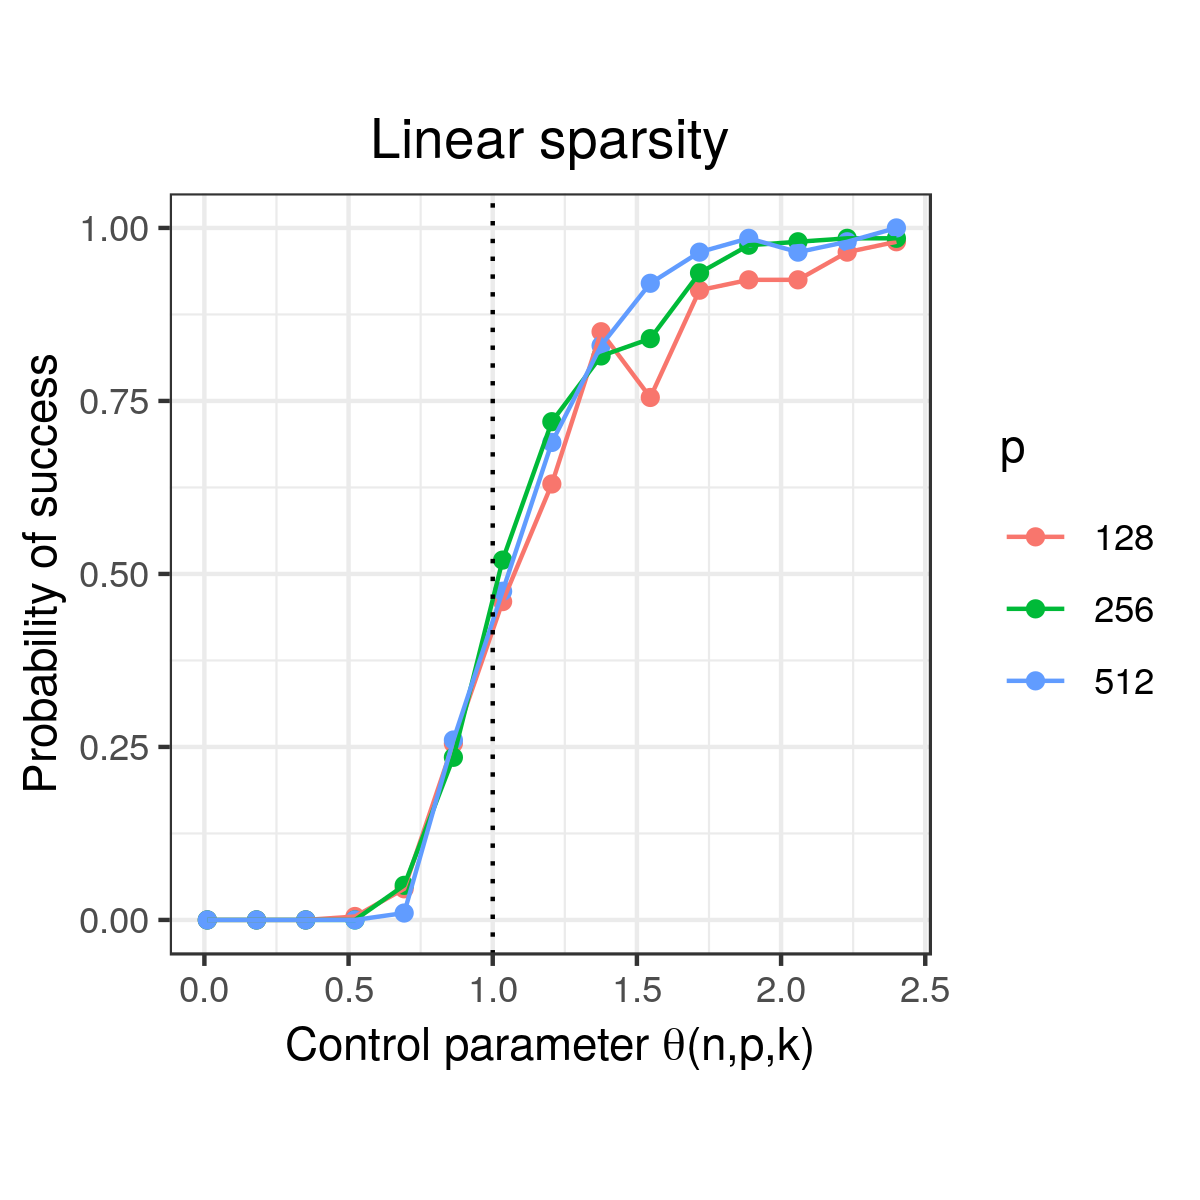
\includegraphics[width=0.9\linewidth]{uniform_linear_sparsity_alpha_1}
    \caption{Linear}
  \end{subfigure}
  \begin{subfigure}{0.32\textwidth}
    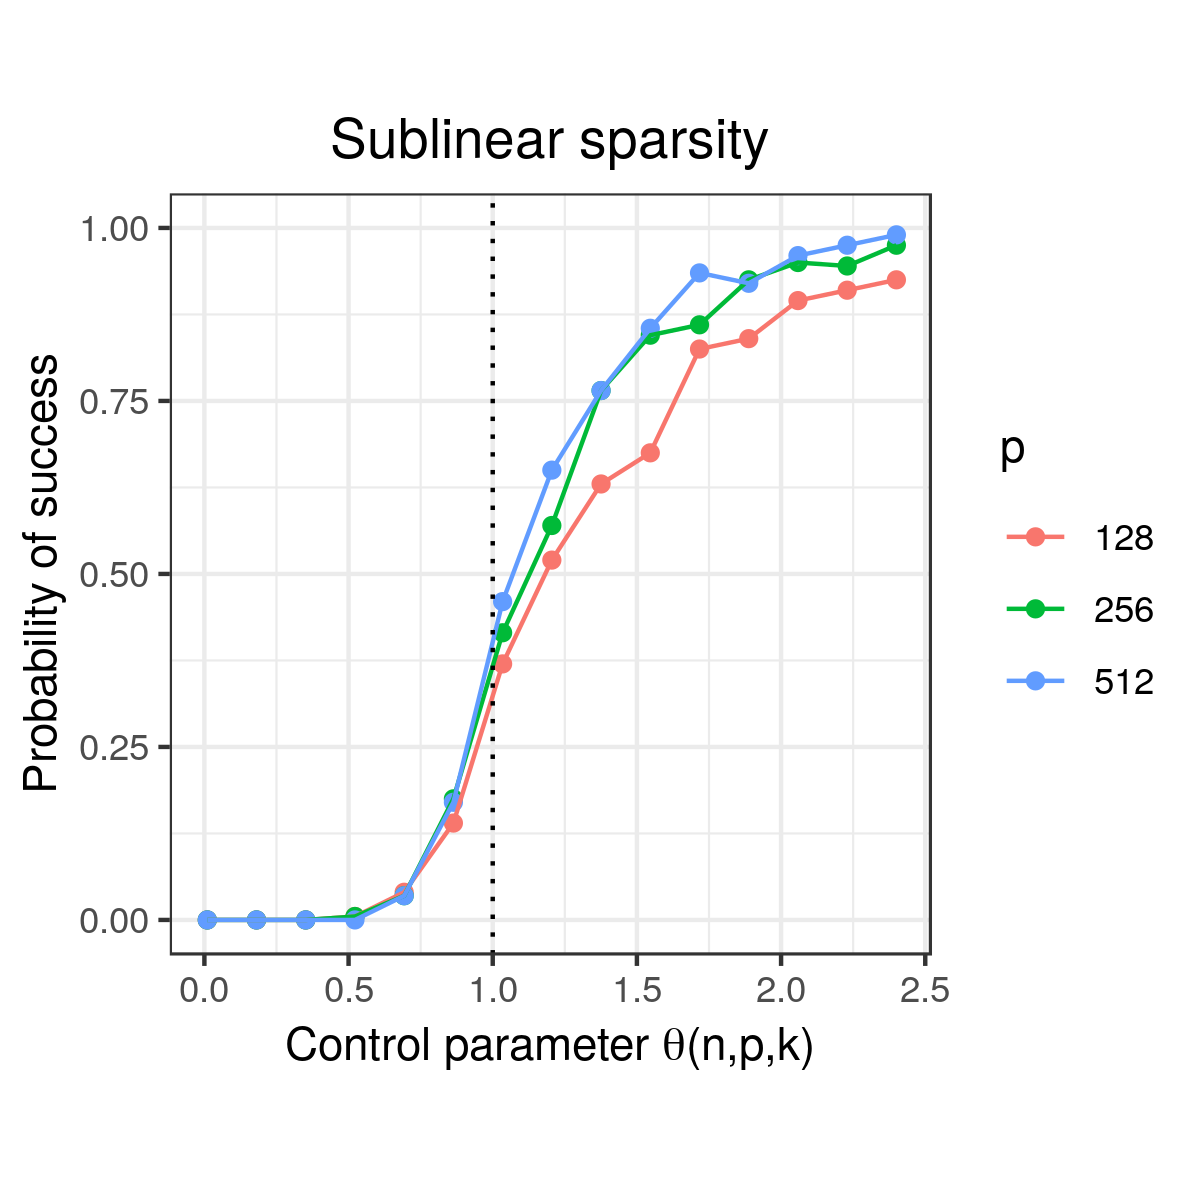
\includegraphics[width=0.9\linewidth]{uniform_sublinear_sparsity_alpha_1}
    \caption{Sublinear}
  \end{subfigure}
  \begin{subfigure}{0.32\textwidth}
    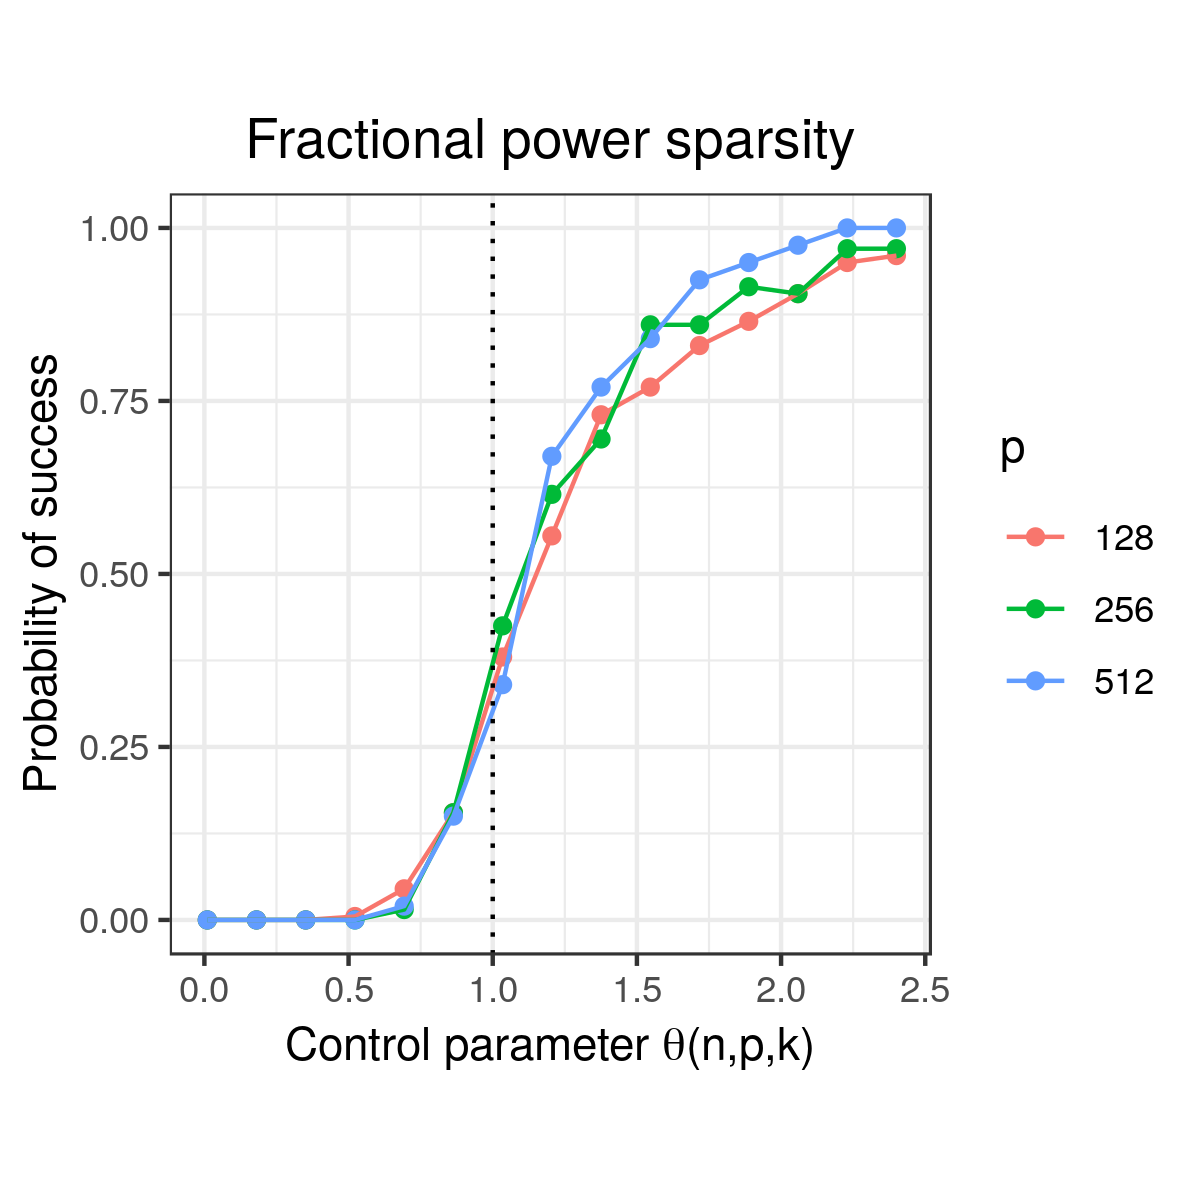
\includegraphics[width=0.9\linewidth]{uniform_fractional_power_sparsity_alpha_1}
    \caption{Fractional power}
  \end{subfigure}
  \caption{Uniform Gaussian ensemble with LASSO}
\end{figure}

\end{frame}

\begin{frame}
\frametitle{Simulations from paper (cont.)}

\begin{figure}[h]
  \centering
  \begin{subfigure}{0.32\textwidth}
    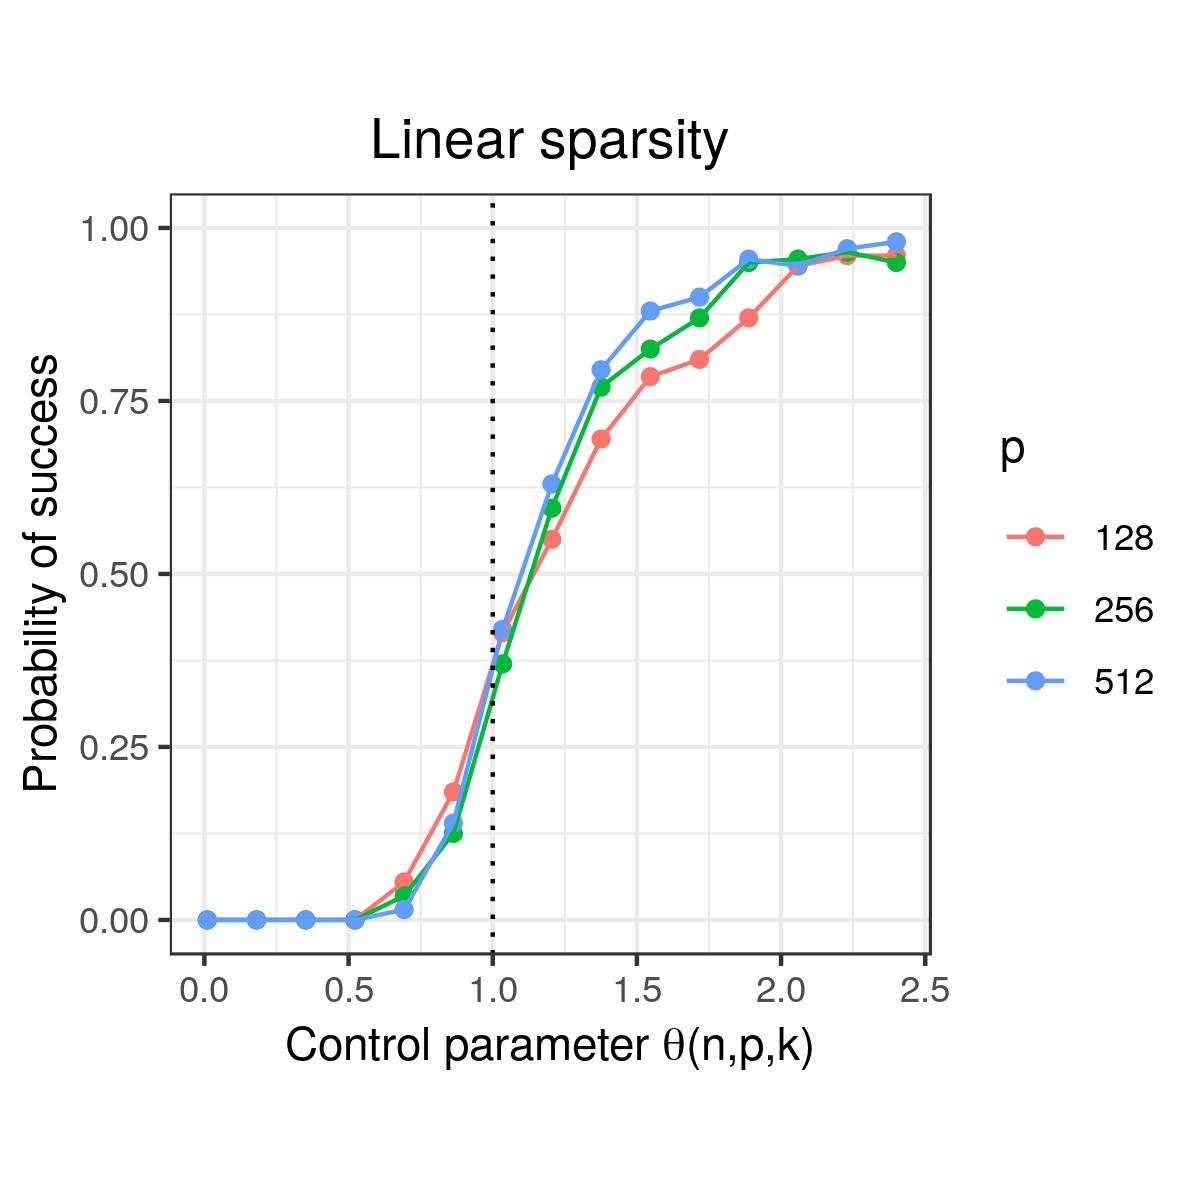
\includegraphics[width=0.9\linewidth]{nonuniform_linear_sparsity_alpha_1}
    \caption{Linear}
  \end{subfigure}
  \begin{subfigure}{0.32\textwidth}
    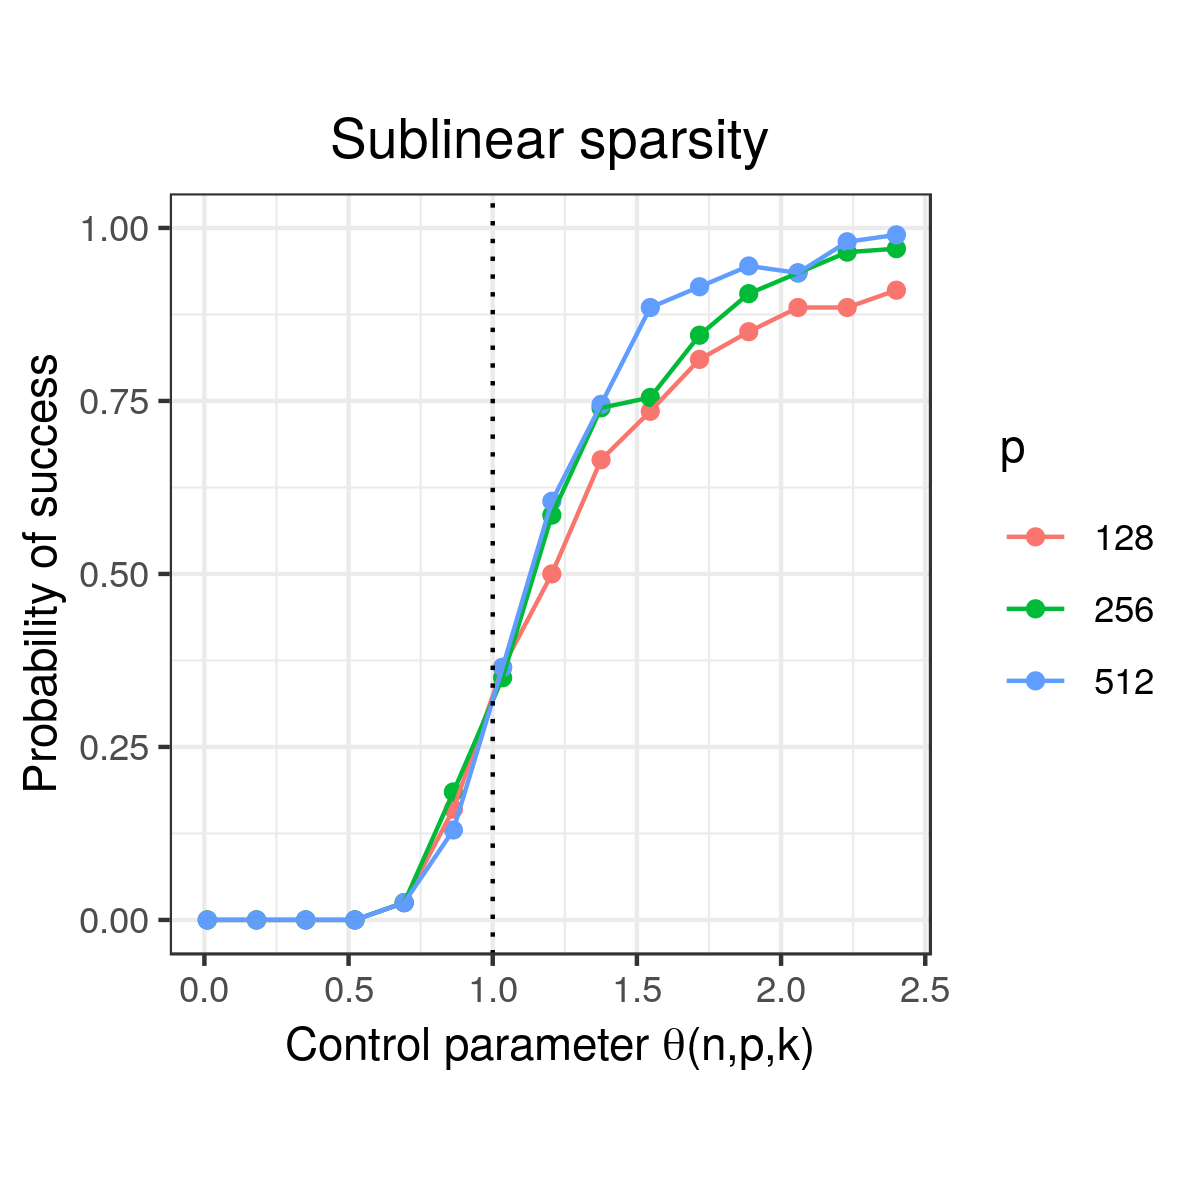
\includegraphics[width=0.9\linewidth]{nonuniform_sublinear_sparsity_alpha_1}
    \caption{Sublinear}
  \end{subfigure}
  \begin{subfigure}{0.32\textwidth}
    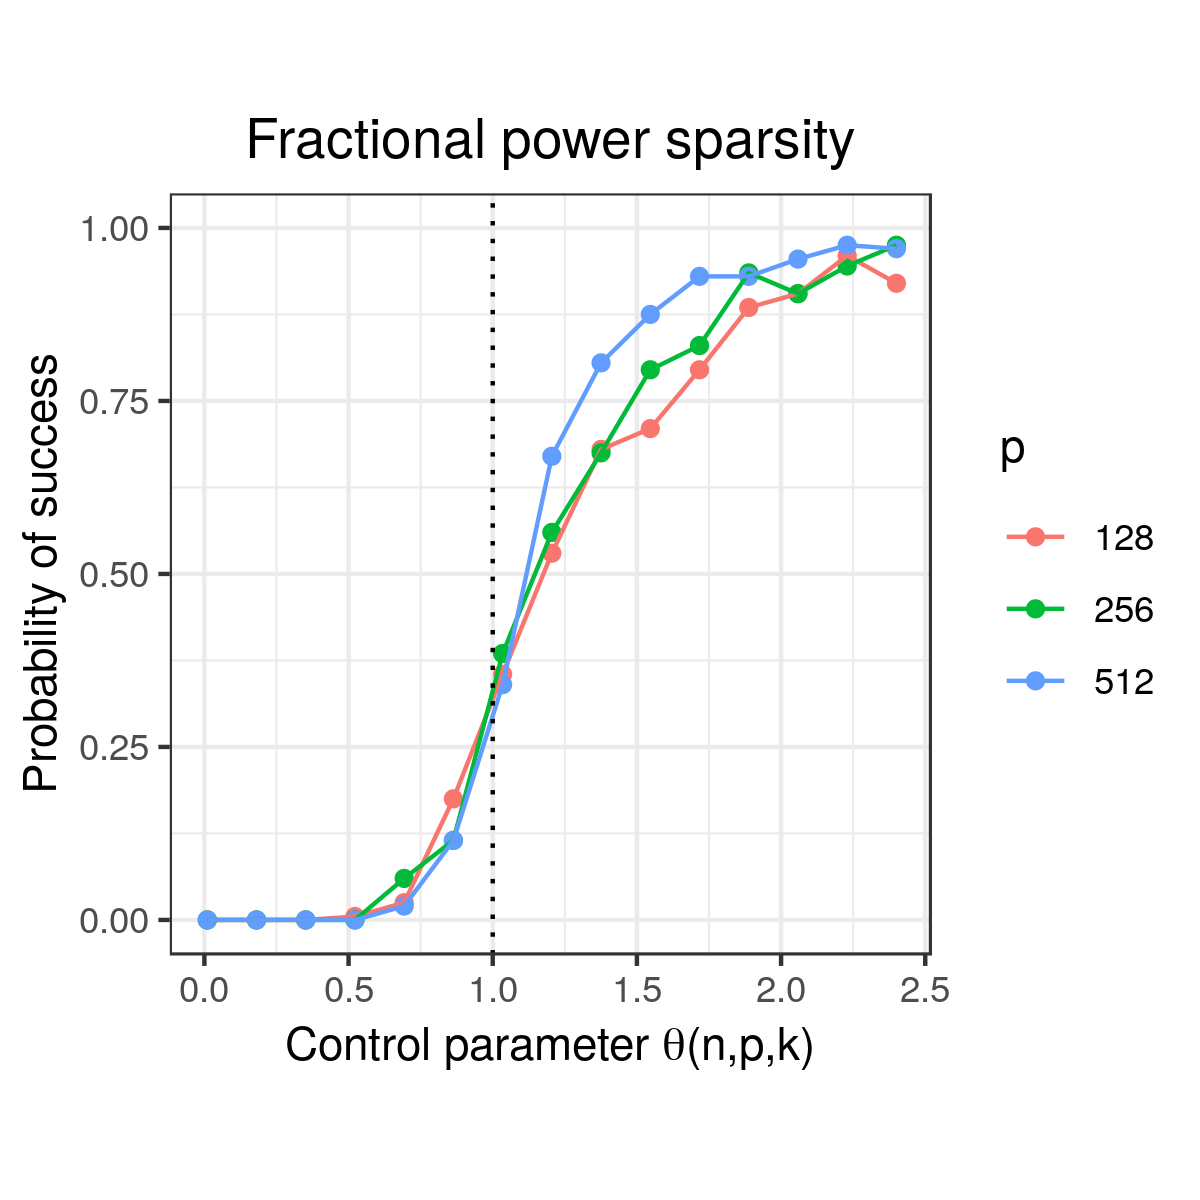
\includegraphics[width=0.9\linewidth]{nonuniform_fractional_power_sparsity_alpha_1}
    \caption{Fractional power}
  \end{subfigure}
  \caption{Non-uniform Gaussian ensemble with LASSO}
\end{figure}

\end{frame}

\begin{frame}
\frametitle{Custom simulations}

\begin{itemize}
\item Same as for uniform Gaussian ensemble simulation from paper, but
  with elastic net penalty ($\alpha = 0.75$ and $\alpha = 0.50$).
\item Unlike with LASSO, have no theoretical guarantees, but
  intuitively expect the theoretical results for LASSO to deteriorate
  as the contribution of the $l_1$-penalty term is diminished (i.e.,
  as $\alpha$ gets smaller).
\item This seems to be what we get!
\end{itemize}

\end{frame}

\begin{frame}
\frametitle{Custom simulations (cont.)}

\begin{figure}[h]
  \centering
  \begin{subfigure}{0.32\textwidth}
    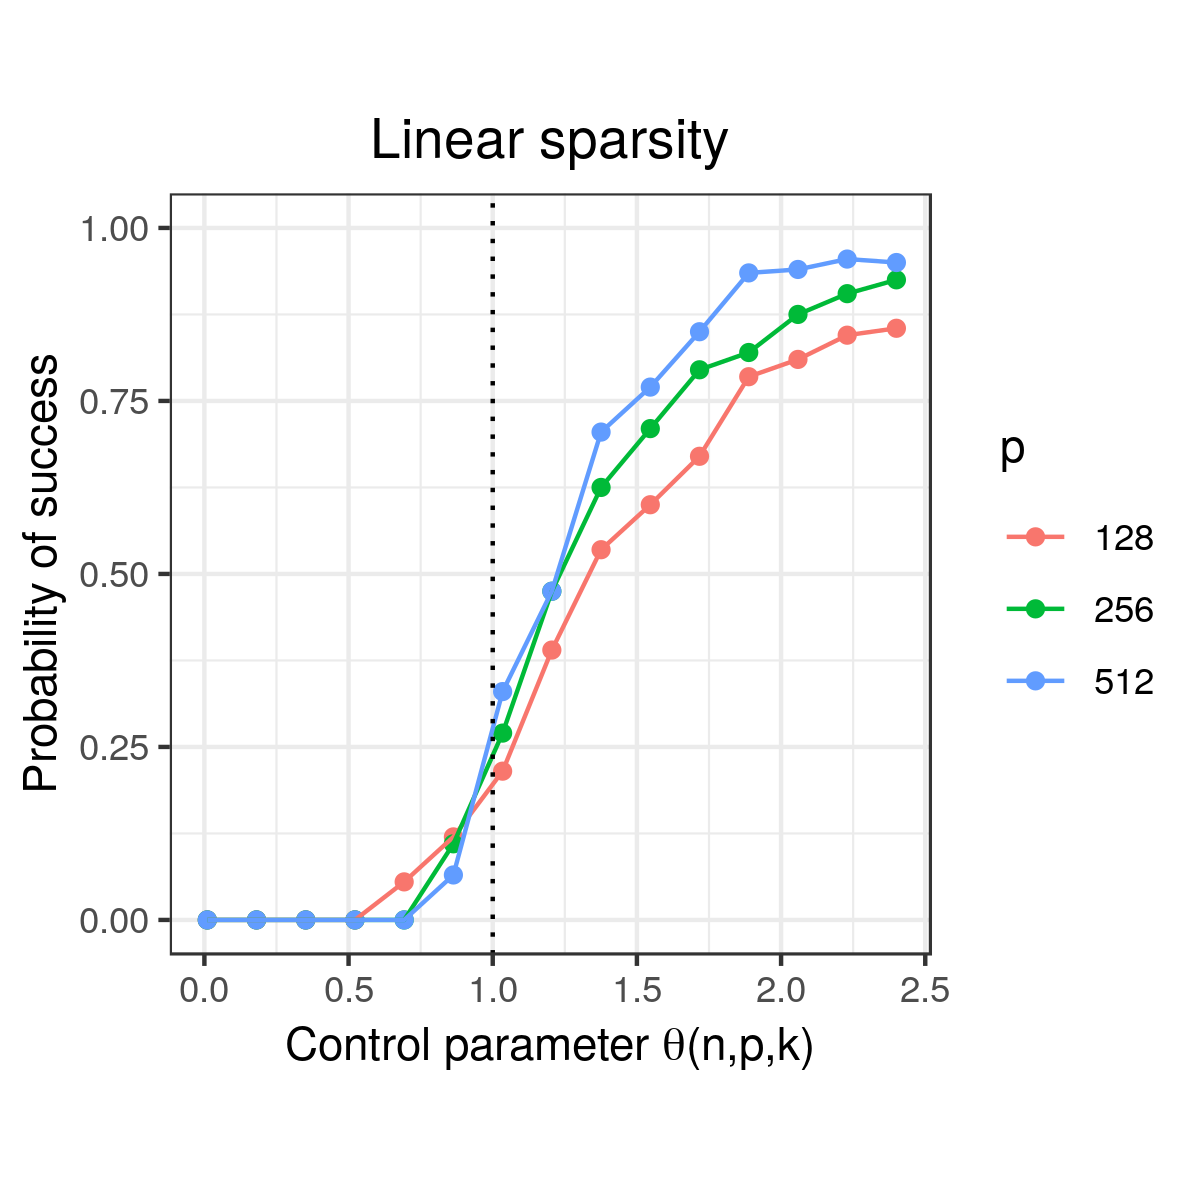
\includegraphics[width=0.9\linewidth]{uniform_linear_sparsity_alpha_075}
    \caption{Linear}
  \end{subfigure}
  \begin{subfigure}{0.32\textwidth}
    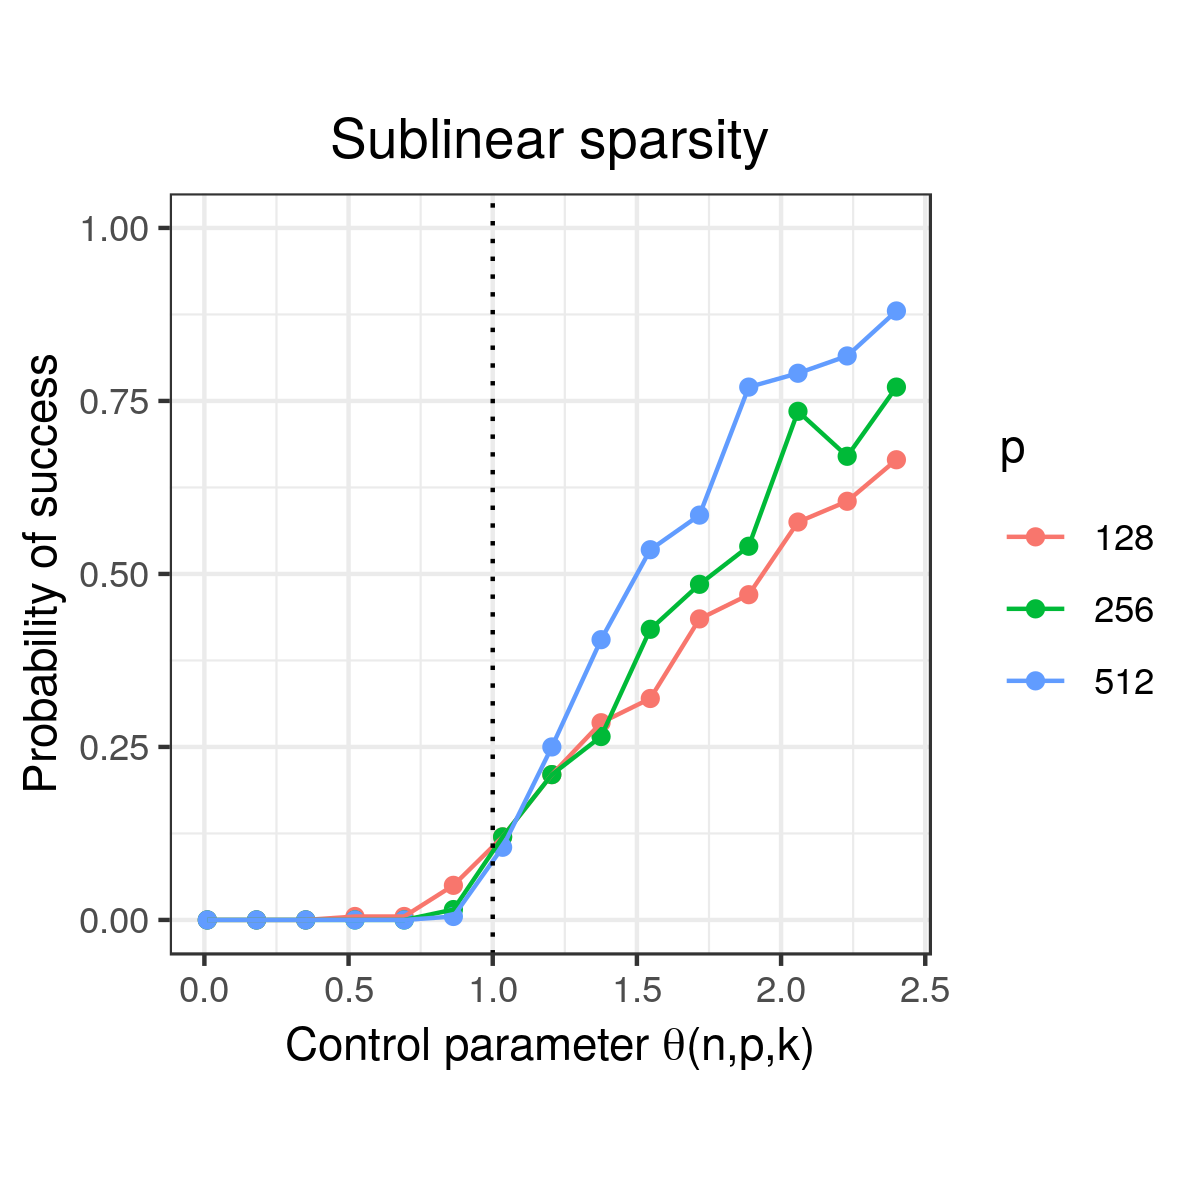
\includegraphics[width=0.9\linewidth]{uniform_sublinear_sparsity_alpha_075}
    \caption{Sublinear}
  \end{subfigure}
  \begin{subfigure}{0.32\textwidth}
    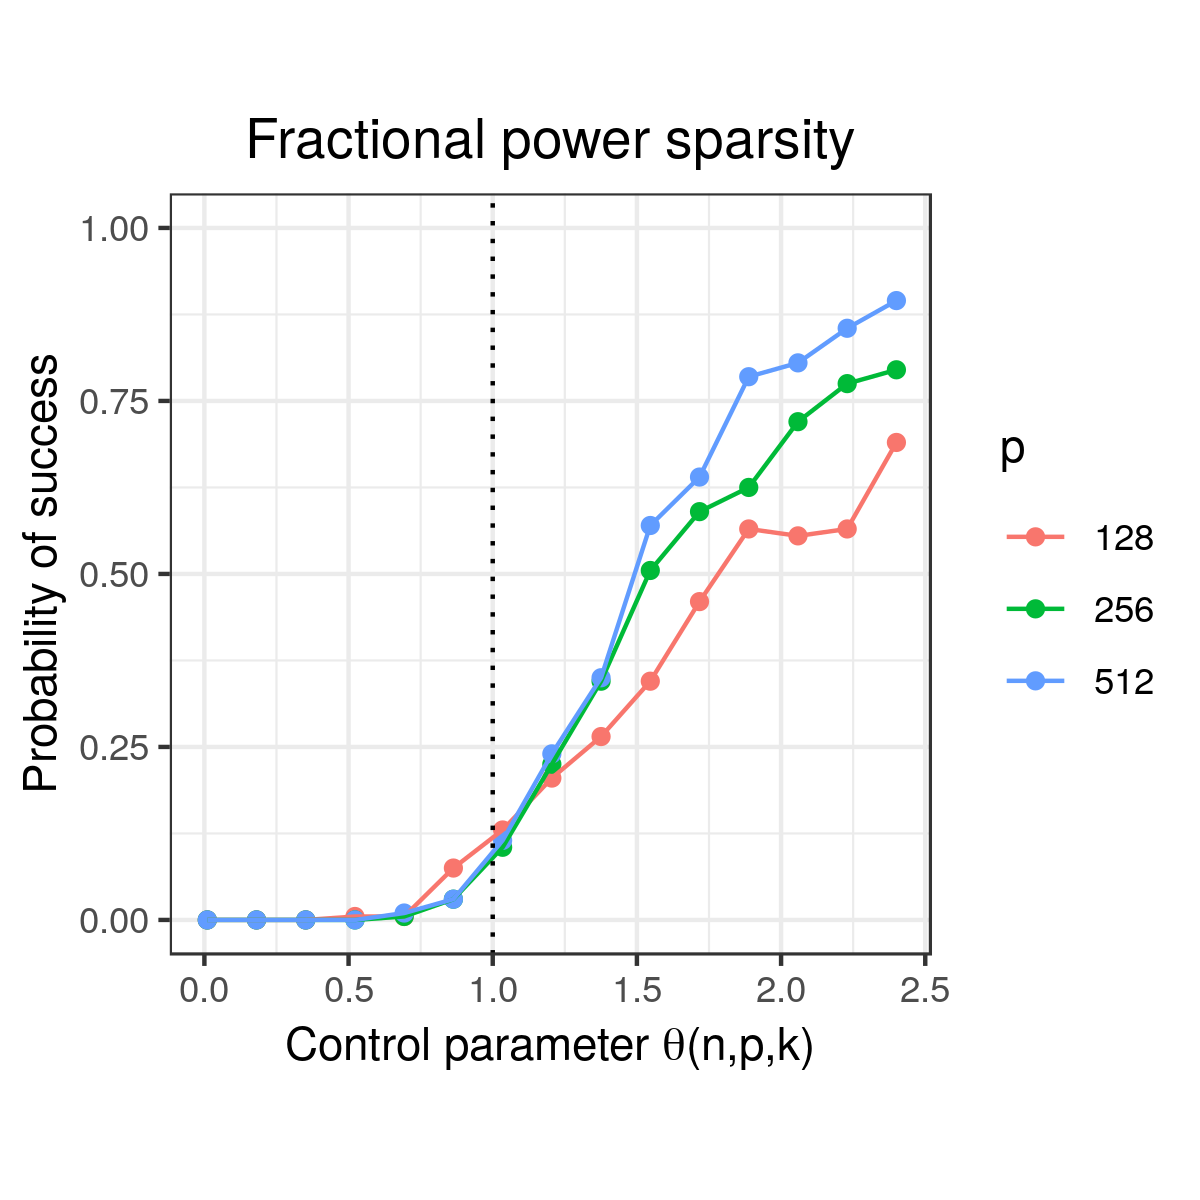
\includegraphics[width=0.9\linewidth]{uniform_fractional_power_sparsity_alpha_075}
    \caption{Fractional power}
  \end{subfigure}
  \caption{Uniform Gaussian ensemble, $\alpha = 0.75$}
\end{figure}

\end{frame}

\begin{frame}
\frametitle{Custom simulations (cont.)}

\begin{figure}[h]
  \centering
  \begin{subfigure}{0.32\textwidth}
    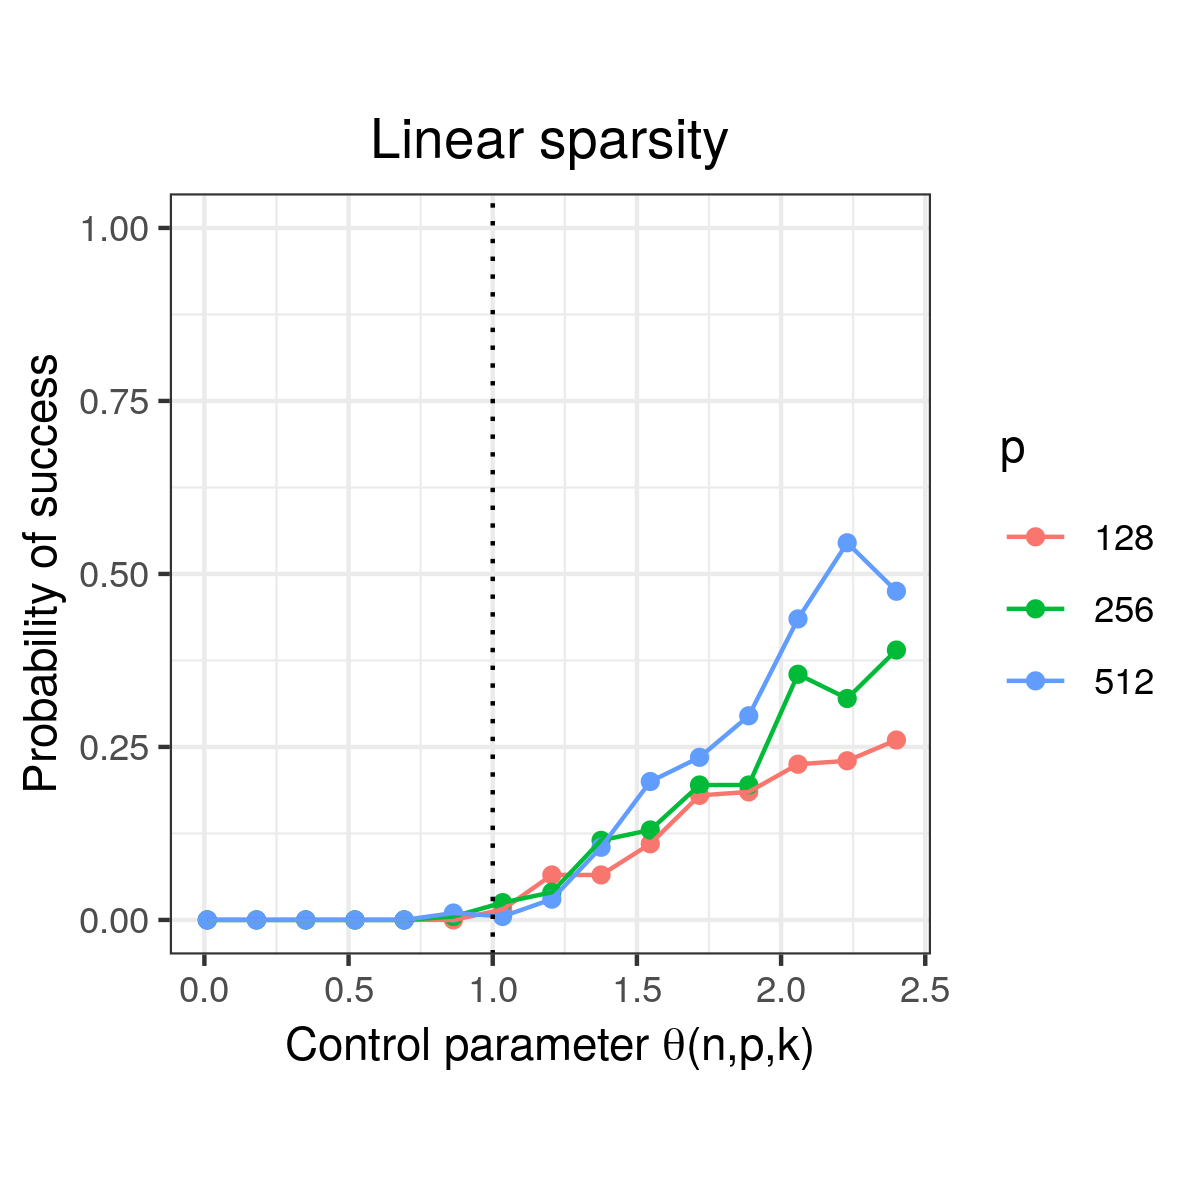
\includegraphics[width=0.9\linewidth]{uniform_linear_sparsity_alpha_050}
    \caption{Linear}
  \end{subfigure}
  \begin{subfigure}{0.32\textwidth}
    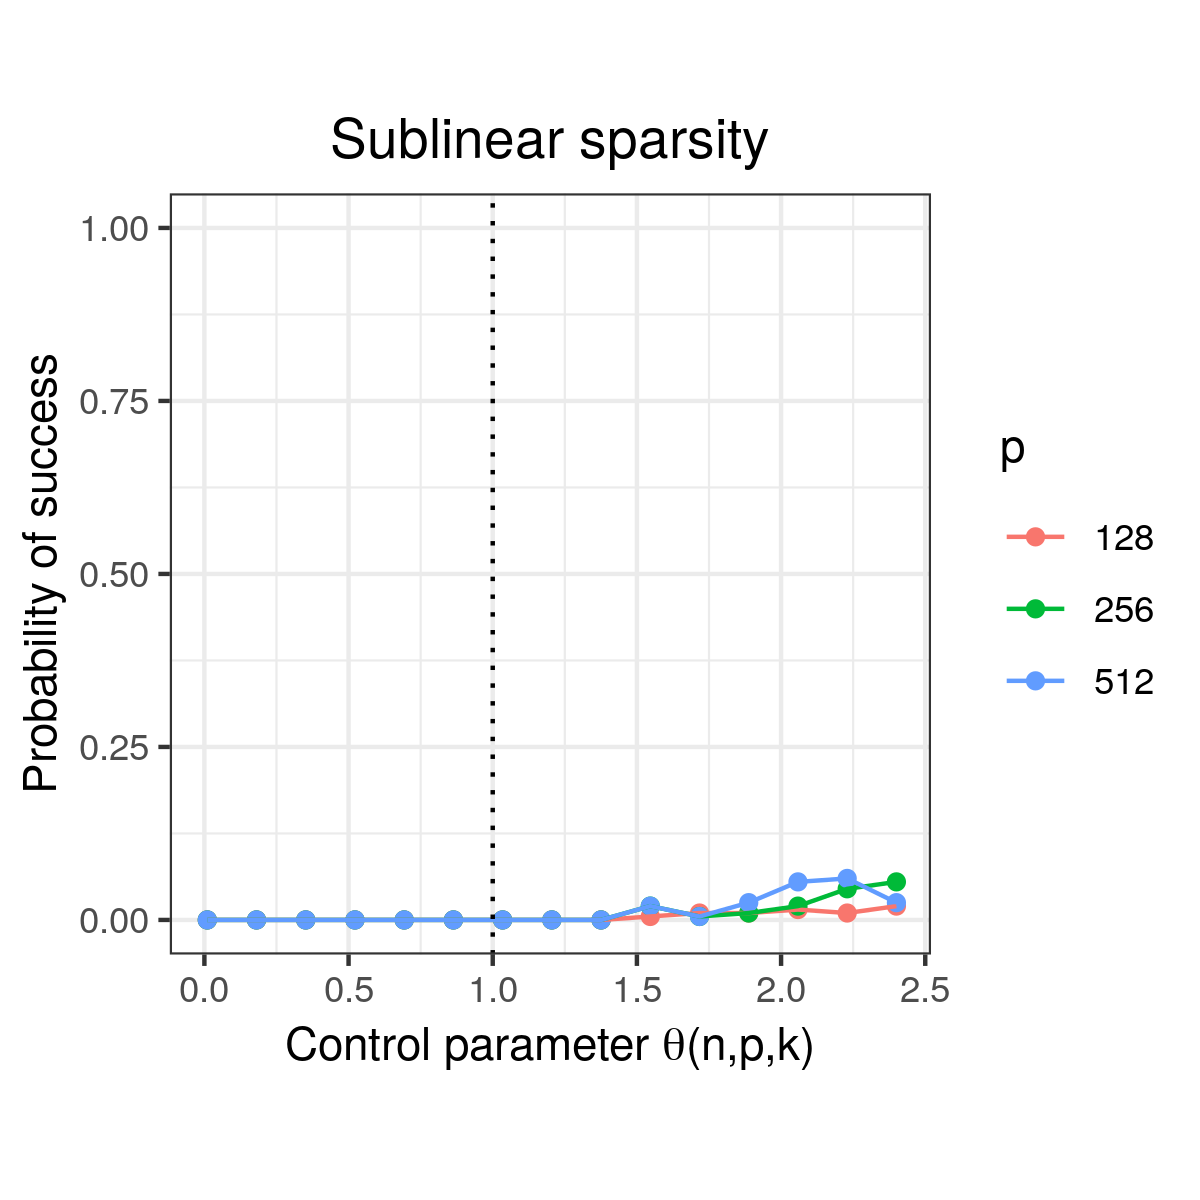
\includegraphics[width=0.9\linewidth]{uniform_sublinear_sparsity_alpha_050}
    \caption{Sublinear}
  \end{subfigure}
  \begin{subfigure}{0.32\textwidth}
    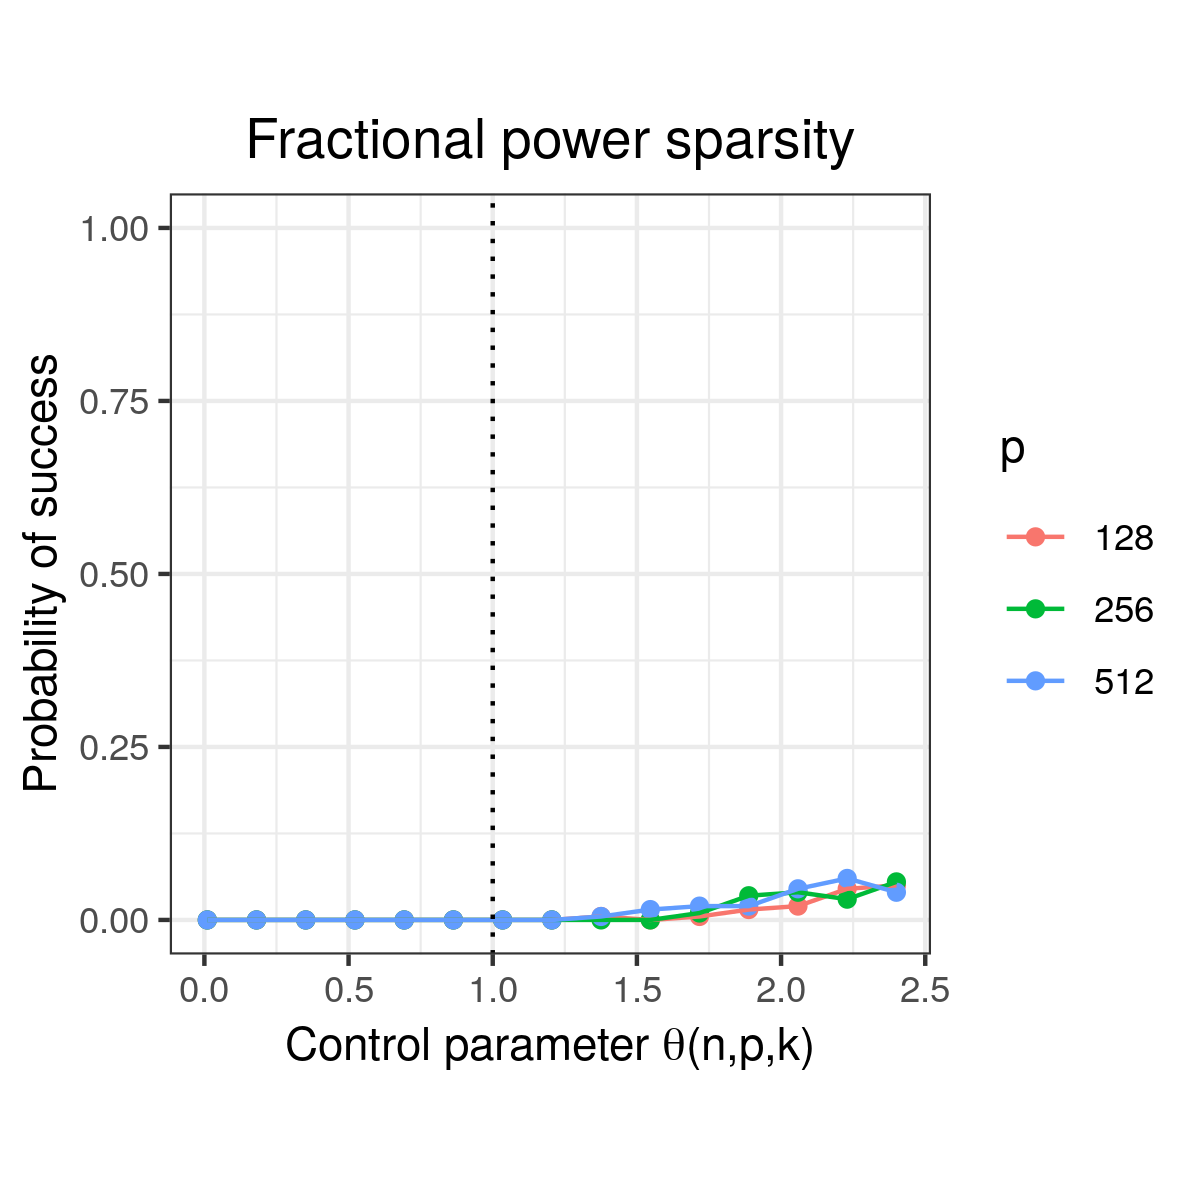
\includegraphics[width=0.9\linewidth]{uniform_fractional_power_sparsity_alpha_050}
    \caption{Fractional power}
  \end{subfigure}
  \caption{Uniform Gaussian ensemble, $\alpha = 0.50$}
\end{figure}

\end{frame}

\end{document}
